\section{Evaluation}
\label{sec:evaluation}

Zur Bewertung des vorgestellten Verfahrens wird besonderes Augenmerk auf schreibintensive Transaktionen, die Performance unterschiedlicher Transaktionstypen und Commit- und Abbruchraten gelegt.
Diese Eigenschaften werden wie zuvor beschrieben mit dem TPC-C Benchmark beobachtet.

\textbf{Schreibintensive Transaktionen:} Die im TPC-C Benchmark enthaltene Payment-Transaktion stellt eine besonders schreibintensive Anwendung dar, weshalb sie für diesen Test verwendet wird.
Dabei wurde zwar der gesamte TPC-C Mix ausgeführt, allerdings wurde nur die besagte Payment-Transaktion beobachtet.

\begin{figure}
	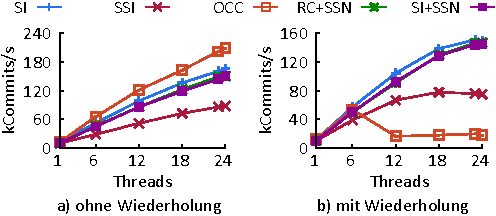
\includegraphics[width=\columnwidth]{img/Figure_3.pdf}
	\caption{Durchsatz der Payment-Transaktion des TPC-C Benchmarks}
	\label{fig:payment}
\end{figure}

Für eine differenzierte Betrachtung wurden zwei verschiedene Testszenarien beobachtet, wobei zum einen sämtliche Transaktionen, die abgebrochen werden mussten ohne eine Wiederholung fallen gelassen wurden.
Zum anderen wurde in einem Test die Performanz des Systems beobachtet wenn die fehlgeschlagenen Transaktionen wiederholt werden bis diese abgeschlossen werden können.
Die Ergebnisse dieser Auswertung sind in Abbildung \ref{fig:payment} grafisch dargestellt.

Dabei fällt auf, dass die Verwendung von Read-Committed in Verbindung mit dem Serial Safety Net einen Durchsatz leistet, der fast doppelt so groß ist wie der der Serializable-Snapshot-Isolation.
Der Grund dafür liegt laut den Autoren darin, dass der Hauptgrund für Transaktionsabbrüche bei der Verwendung von SSI in dem sogenannten Temporal Skew liegt.
Dabei versucht eine Transaktion eine Version zu überschreiben, welche nach ihrem Snapshot erstellt wurde, was bei SSI nicht zulässig ist.
RC hat damit kein Problem, da jederzeit auf die neueste Version zugegriffen wird, was sich auch durch die Erweiterung durch das SSN nicht ändert.

Außerdem ist zu erkennen, dass auch die Snapshot-Isolation in Verbindung mit dem SSN eine hervorragende Performanz in beiden Testfällen besitzt.

Die Verwendung der Optimistic-Concurrency-Control zeigt bei dem Test ohne Wiederholungen die beste Performanz, da ein Großteil des Verwaltungsaufwandes der anderen CC-Verfahren entfällt.
Wird allerdings verlangt, dass die Transaktionen nach einem Abbruch wiederholt werden müssen, so sinkt der Durchsatz der OCC weit unter den Durchsatz der anderen CC-Verfahren, da die Zahl der zu wiederholenden Transaktionen so hoch ist, dass bei stark nebenläufigen Transaktionen die Performanz einbricht.

\textbf{Performanz unterschiedlicher Transaktionsarten:} Zum Testen des Durchsatzes der verschiedenen Transaktionstypen des TPC-C Benchmarks wurden die vorher untersuchten Verfahren mit dem aus der TPC-C Spezifikation entnommenen Idealwert verglichen.
Der Test wurde auf einer Maschine mit 24 Threads und ohne Wiederholen von abgebrochenen Transaktionen durchgeführt, wodurch das in Abbildung \ref{fig:breakdown} dargestellte Ergebnis erzielt wurde.

\begin{figure}
	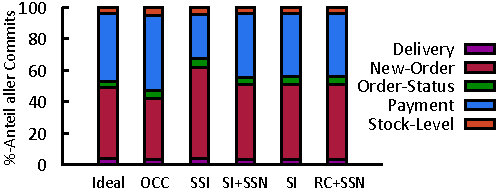
\includegraphics[width=\columnwidth]{img/Figure_4.pdf}
	\caption{Anteil des Durchsatzes der verschiedenen Transaktionstypen des TPC-C Benchmarks}
	\label{fig:breakdown}
\end{figure}

Die Grafik zeigt den Anteil der erfolgreich abgeschlossenen Transaktionen jedes Typs an der Gesamtzahl der erfolgreich abgeschlossenen Transaktionen.
Besonderes Augenmerk fällt hierbei auf die Payment-Transaktion, welche einen besonders schreibintensiven Anwendungsfall abbildet.

Hier liefert die OCC einen sehr hohen Durchsatz, was darauf schließen lässt, dass das ursprünglich in Silo implementierte System besonders gut für schreiblastige Applikationen geeignet ist, nicht jedoch für Transaktionen, die zusätzlich viele Leseoperationen durchführen.
Außerdem fällt auf, dass die SSI eine sehr schlechte Leistung für schreibintensive Anwendungen liefert, wodurch grundsätzlich die Ergebnisse aus dem vorhergehenden Abschnitt bestätigt werden.
Bemerkenswert ist, dass die Erweiterung der SI durch das SSN keine nennenswerte Änderung an der dargestellten Verteilung bewirkt, wodurch erkennbar ist, dass das SSN einen gleichmäßigen Einfluss auf die Performanz der verschiedenen Transaktionstypen hat und nicht eine besondere Transaktionsart wie beispielsweise leseintensive Transaktionstypen besonders beeinflusst.
Ebenfalls vielversprechend ist die Tatsache, dass beide Varianten des SSN sehr nah an der durch die TPC-C Spezifikation vorgesehenen Idealverteilung liegen, wodurch sichergestellt ist, dass es sich dabei um ein ausgewogenes Verfahren handelt, mit dem eine Vielzahl von Anwendungsfällen effizient umgesetzt werden kann.

\textbf{Commit- und Abbruchraten:} Für die Untersuchung der Commit- und Abbruchraten wurde wieder der gesamte TPC-C Mix beobachtet, wobei die Untersuchungen jeweils mit und ohne Wiederholung fehlgeschlagener Transaktionen durchgeführt wurden.

\begin{figure*}
	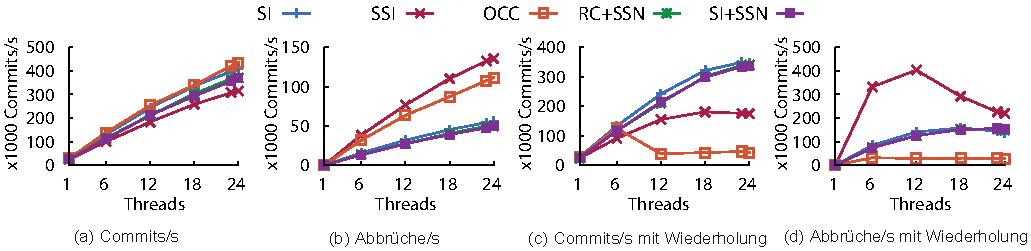
\includegraphics[width=\textwidth]{img/Figure_5_original.pdf}
	\caption{Commit- und Abbruchraten des TPC-C Benchmarks mit und ohne Wiederholung abgebrochener Transaktionen}
	\label{fig:commit_abort}
\end{figure*}

Die dazu in Abbildung \ref{fig:commit_abort} dargestellten Ergebnisse geben dazu Auskunft über die diesbezüglichen Eigenschaften der unterschiedlichen Verfahren.
Die in a und c dargestellten Commitraten bestätigen die Ergebnisse, die zuvor bei der Untersuchung der Payment-Transaktion festgestellt wurden, da sich der gesamte TPC-C Mix sehr ähnlich wie diese verhält.
In a und b dargestellten Ergebnisse zeigen, dass alle Verfahren gut mit der Anzahl der Threads skalieren, wenn fehlgeschlagene Transaktionen nicht wiederholt werden.
Außerdem lässt sich in b erkennen, dass SSI und OCC fast doppelt so oft Transaktionen abbrechen wie die Varianten des SSN.
Aufgrund der kleinen Grafik lässt es sich zwar schwer erkennen, allerdings schneidet RC+SSN in diesem Fall minimal besser ab als SI+SSN, da dieses einige Transaktionspläne erlaubt, welche von letzterem verboten werden.

In Teil d der Abbildung fällt auf, dass SSI eine weitaus höhere Abbruchrate als die anderen Verfahren besitzt.
Zunächst verwundern dürfte außerdem die Tatsache, dass OCC in dieser Darstellung die geringste Abbruchrate besitzt, was allerdings darin begründet ist, dass das in Silo eingesetzte Verfahren einen hohen Overhead beim Einfügen von Indexeinträgen verursacht wodurch nur wenige Transaktionen pro Sekunde betrachtet werden, was sich beispielsweise auch in c widerspiegelt.

\textbf{Zulässige Transaktionspläne:} Die Unterschiede zwischen den untersuchten Verfahren zur Sicherung der Serialisierbarkeit werden besonders deutlich, wenn ein paar beispielhafte Abhängigkeitsstrukturen in Transaktionsplänen verglichen werden.
Dazu sind in Abbildung \ref{fig:transaktionsplan_formen} einige Transaktionspläne aufgezeigt und dazu vermerkt, ob jeweils das SSN, 2PL oder SSI dies Pläne akzeptiert oder verwirft.
Dabei kann angenommen werden, dass in den entsprechenden Graphen keine Abhängigkeitszyklen enthalten sind und in einem perfekten System somit keiner der Pläne verworfen werden müsste.

\begin{figure*}
	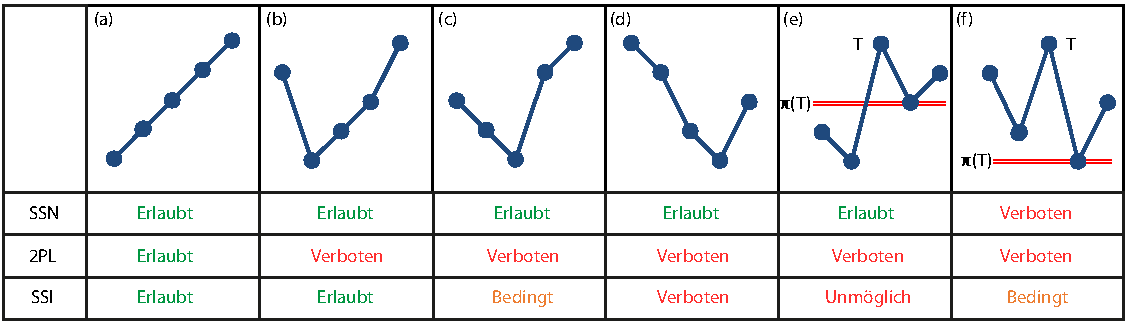
\includegraphics[width=\textwidth]{img/Figure_6.pdf}
	\caption{Einige Beispiele für mögliche Transaktionspläne und ob diese von SSN, 2PL oder SSI akzeptiert werden}
	\label{fig:transaktionsplan_formen}
\end{figure*}

Es wird direkt deutlich, dass SSN wesentlich mehr Pläne zulässt als die anderen Verfahren, es verwirft sogar nur den Plan f, da dieser als einziger die Ungleichung \ref{eq:ausschlussfenster_kurz} aus Kapitel \ref{sec:ssn} erfüllt und somit nicht zulässig ist.

Das 2PL verbietet dagegen sämtliche Pläne abgesehen von Plan a, da dieses Verfahren das Vorkommen von Back-Edges vollständig verbietet und alle anderen Pläne solche Abhängigkeiten enthalten.

Die SSI erlaubt grundsätzlich die Pläne a und b und verbietet in jedem Fall den Plan d.
Ein Fall wie ihn Plan c zeigt, wird nur von SSI akzeptiert, wenn die Transaktion ganz links ausschließlich Leseoperationen enthält und schon ausreichend alt ist.
Der Transaktionsplan e kann bei der Verwendung von SI erst gar nicht auftreten und ist somit auch bei der Verwendung von SSI unmöglich.
Grundsätzlich wird der Plan f zwar akzeptiert, ist aber die Transaktion $T$ mit seinem Vorgänger durch eine harmlose Anti-Abhängigkeit verbunden, so wird auch dieser Plan von SSI verworfen.

Somit sollte deutlich werden, dass das SSN viele zulässige Transaktionspläne erlaubt, die die anderen Verfahren unnötigerweise verwerfen, wodurch ebenfalls ein deutlicher Performanzgewinn begründet werden kann.